\documentclass[12pt]{article}
\usepackage[left=1cm, right=1cm, top=2cm,bottom=1.5cm]{geometry} 

\usepackage[parfill]{parskip}
\usepackage[utf8]{inputenc}
\usepackage[T2A]{fontenc}
\usepackage[russian]{babel}
\usepackage{enumitem}
\usepackage[normalem]{ulem}
\usepackage{amsfonts, amsmath, amsthm, amssymb, mathtools,xcolor}
\usepackage{blkarray}

\usepackage{tabularx}
\usepackage{hhline}

\usepackage{accents}
\usepackage{fancyhdr}
\pagestyle{fancy}
\renewcommand{\headrulewidth}{1.5pt}
\renewcommand{\footrulewidth}{1pt}

\usepackage{graphicx}
\usepackage[figurename=Рис.]{caption}
\usepackage{subcaption}
\usepackage{float}

%%Наименование папки откуда забирать изображения
\graphicspath{ {./images/} }

%%Изменение формата для ввода доказательства
\renewcommand{\proofname}{$\square$  \nopunct}
\renewcommand\qedsymbol{$\blacksquare$}

%%Изменение отступа на таблицах
\addto\captionsrussian{%
	\renewcommand{\proofname}{$\square$ \nopunct}%
}
%% Римские цифры
\newcommand{\RN}[1]{%
	\textup{\uppercase\expandafter{\romannumeral#1}}%
}

%% Для удобства записи
\newcommand{\MR}{\mathbb{R}}
\newcommand{\MC}{\mathbb{C}}
\newcommand{\MQ}{\mathbb{Q}}
\newcommand{\MN}{\mathbb{N}}
\newcommand{\MZ}{\mathbb{Z}}
\newcommand{\MTB}{\mathbb{T}}
\newcommand{\MTI}{\mathbb{I}}
\newcommand{\MI}{\mathrm{I}}
\newcommand{\MCI}{\mathcal{I}}
\newcommand{\MJ}{\mathrm{J}}
\newcommand{\MH}{\mathrm{H}}
\newcommand{\MT}{\mathrm{T}}
\newcommand{\MU}{\mathcal{U}}
\newcommand{\MV}{\mathcal{V}}
\newcommand{\MB}{\mathcal{B}}
\newcommand{\MF}{\mathcal{F}}
\newcommand{\MW}{\mathcal{W}}
\newcommand{\ML}{\mathcal{L}}
\newcommand{\MP}{\mathcal{P}}
\newcommand{\VN}{\varnothing}
\newcommand{\VE}{\varepsilon}
\newcommand{\dx}{\, dx}
\newcommand{\dy}{\, dy}
\newcommand{\dz}{\, dz}
\newcommand{\dd}{\, d}


\theoremstyle{definition}
\newtheorem{defn}{Опр:}
\newtheorem{rem}{Rm:}
\newtheorem{prop}{Утв.}
\newtheorem{exrc}{Упр.}
\newtheorem{problem}{Задача}
\newtheorem{lemma}{Лемма}
\newtheorem{theorem}{Теорема}
\newtheorem{corollary}{Следствие}

\newenvironment{cusdefn}[1]
{\renewcommand\thedefn{#1}\defn}
{\enddefn}

\DeclareRobustCommand{\divby}{%
	\mathrel{\text{\vbox{\baselineskip.65ex\lineskiplimit0pt\hbox{.}\hbox{.}\hbox{.}}}}%
}
\DeclareRobustCommand{\ndivby}{\mkern-1mu\not\mathrel{\mkern4.5mu\divby}\mkern1mu}


%Короткий минус
\DeclareMathSymbol{\SMN}{\mathbin}{AMSa}{"39}
%Длинная шапка
\newcommand{\overbar}[1]{\mkern 1.5mu\overline{\mkern-1.5mu#1\mkern-1.5mu}\mkern 1.5mu}
%Функция знака
\DeclareMathOperator{\sgn}{sgn}

%Функция ранга
\DeclareMathOperator{\rk}{\text{rk}}
\DeclareMathOperator{\diam}{\text{diam}}


%Обозначение константы
\DeclareMathOperator{\const}{\text{const}}

\DeclareMathOperator{\codim}{\text{codim}}

\DeclareMathOperator*{\dsum}{\displaystyle\sum}
\newcommand{\ddsum}[2]{\displaystyle\sum\limits_{#1}^{#2}}
\newcommand{\ddssum}[2]{\displaystyle\smashoperator{\sum\limits_{#1}^{#2}}}
\newcommand{\ddlsum}[2]{\displaystyle\smashoperator[l]{\sum\limits_{#1}^{#2}}}
\newcommand{\ddrsum}[2]{\displaystyle\smashoperator[r]{\sum\limits_{#1}^{#2}}}

%Интеграл в большом формате
\DeclareMathOperator{\dint}{\displaystyle\int}
\newcommand{\ddint}[2]{\displaystyle\int\limits_{#1}^{#2}}
\newcommand{\ssum}[1]{\displaystyle \sum\limits_{n=1}^{\infty}{#1}_n}

\newcommand{\smallerrel}[1]{\mathrel{\mathpalette\smallerrelaux{#1}}}
\newcommand{\smallerrelaux}[2]{\raisebox{.1ex}{\scalebox{.75}{$#1#2$}}}

\newcommand{\smallin}{\smallerrel{\in}}
\newcommand{\smallnotin}{\smallerrel{\notin}}

\newcommand*{\medcap}{\mathbin{\scalebox{1.25}{\ensuremath{\cap}}}}%
\newcommand*{\medcup}{\mathbin{\scalebox{1.25}{\ensuremath{\cup}}}}%

\makeatletter
\newcommand{\vast}{\bBigg@{3.5}}
\newcommand{\Vast}{\bBigg@{5}}
\makeatother

%Промежуточное значение для sup\inf, поскольку они имеют разную высоту
\newcommand{\newsup}{\mathop{\smash{\mathrm{sup}}}}
\newcommand{\newinf}{\mathop{\mathrm{inf}\vphantom{\mathrm{sup}}}}

%Скалярное произведение
\newcommand{\inner}[2]{\left\langle #1, #2 \right\rangle }
\newcommand{\linsp}[1]{\left\langle #1 \right\rangle }
\newcommand{\linmer}[2]{\left\langle #1 \vert #2\right\rangle }

%Подпись символов снизу
\newcommand{\ubar}[1]{\underaccent{\bar}{#1}}

%%Шапка для букв сверху
\newcommand{\wte}[1]{\widetilde{#1}}
\newcommand{\wht}[1]{\widehat{#1}}
\newcommand{\ovl}[1]{\overline{#1}}


%%Трансформация Фурье
\newcommand{\fourt}[1]{\mathcal{F}\left(#1\right)}
\newcommand{\ifourt}[1]{\mathcal{F}^{-1}\left(#1\right)}

%%Символ вектора
\newcommand{\vecm}[1]{\overrightarrow{#1\,}}

%%Пространстов матриц
\newcommand{\matsq}[1]{\operatorname{Mat}_{#1}}
\newcommand{\mat}[2]{\operatorname{Mat}_{#1, #2}}

%Оператор для действ и мнимых чисел
\DeclareMathOperator{\IM}{\operatorname{Im}}
\DeclareMathOperator{\RE}{\operatorname{Re}}
\DeclareMathOperator{\li}{\operatorname{li}}
\DeclareMathOperator{\GL}{\operatorname{GL}}
\DeclareMathOperator{\SL}{\operatorname{SL}}
\DeclareMathOperator{\Char}{\operatorname{char}}
\DeclareMathOperator\Arg{Arg}
\DeclareMathOperator\ord{ord}

%Оператор для образа
\DeclareMathOperator{\Ima}{Im}

%Делимость чисел
\newcommand{\modn}[3]{#1 \equiv #2 \; (\bmod \; #3)}
\newcommand{\nmodn}[3]{#1 \not\equiv #2 \; (\bmod \; #3)}

%%Взятие в скобки, модули и норму
\newcommand{\parfit}[1]{\left( #1 \right)}
\newcommand{\modfit}[1]{\left| #1 \right|}
\newcommand{\sqparfit}[1]{\left\{ #1 \right\}}
\newcommand{\normfit}[1]{\left\| #1 \right\|}

%%Функция для обозначения равномерной сходимости по множеству
\newcommand{\uconv}[1]{\overset{#1}{\rightrightarrows}}
\newcommand{\uconvm}[2]{\overset{#1}{\underset{#2}{\rightrightarrows}}}


%%Функция для обозначения нижнего и верхнего интегралов
\def\upint{\mathchoice%
	{\mkern13mu\overline{\vphantom{\intop}\mkern7mu}\mkern-20mu}%
	{\mkern7mu\overline{\vphantom{\intop}\mkern7mu}\mkern-14mu}%
	{\mkern7mu\overline{\vphantom{\intop}\mkern7mu}\mkern-14mu}%
	{\mkern7mu\overline{\vphantom{\intop}\mkern7mu}\mkern-14mu}%
	\int}
\def\lowint{\mkern3mu\underline{\vphantom{\intop}\mkern7mu}\mkern-10mu\int}

%%След матрицы
\DeclareMathOperator*{\tr}{tr}

\makeatletter
\renewcommand*\env@matrix[1][*\c@MaxMatrixCols c]{%
	\hskip -\arraycolsep
	\let\@ifnextchar\new@ifnextchar
	\array{#1}}
\makeatother


%% Переопределение функции хи, чтобы выглядела более приятно
\makeatletter
\@ifdefinable\@latex@chi{\let\@latex@chi\chi}
\renewcommand*\chi{{\@latex@chi\smash[t]{\mathstrut}}} % want only bottom half of \mathstrut
\makeatletter

\setcounter{MaxMatrixCols}{20}
\begin{document}
\lhead{Математический анализ - \RN{4}}
\chead{Шапошников С.В.}
\rhead{Лекция - 2}

\section*{Критерий интегрируемости. Теорема Фубини}

\begin{theorem}
	Пусть $f$ - ограниченная функция на замкнутом бруске $\MI$. $f$ - интегрируема по Риману на $\MI$ тогда и только тогда, когда $\exists$ последовательности ступенчатых функций $h_n, g_n$ такие, что:
	\begin{enumerate}[label=\arabic*)]
		\item $h_n(x) \leq h_{n+1}(x); \,  g_{n+1}(x) \leq g_n(x),\, \forall n$;
		\item $h_n(x) \leq f(x) \leq g_n(x),\, \forall n$;
		\item $\int_{\MI}g_n(x)dx - \int_{\MI}h_n(x)dx \xrightarrow[n \to \infty]{} 0$;
	\end{enumerate}
\end{theorem}
\begin{rem}
	Отметим, что это фактически критерий Дарбу, изложенный на языке функций, где равномерная сходимость заменена на монотонную последовательность.
\end{rem}

\begin{proof}\hfill\\
	$(\Leftarrow)$ Пусть $(\MTB,\xi)$ - отмеченное разбиение, $h_n \leq f \leq g_n$, следовательно (объемы брусков $\geq 0$):
	$$
		\sigma(h_n,\MTB,\xi) \leq \sigma(f,\MTB,\xi) \leq \sigma(g_n, \MTB, \xi) 
	$$
	Заметим, что последовательность интегралов от $h_n$ не убывает, а $g_n$ не возрастает:
	$$
		\ddint{\MI}{}h_n(x)dx \leq \ddint{\MI}{}h_{n+1}(x)dx, \quad \ddint{\MI}{}g_{n+1}(x)dx \leq \ddint{\MI}{}g_n(x)dx
	$$
	Поскольку $f$ - ограниченна, то эти последовательности ограниченны $\Rightarrow$ у монотонных, ограниченных последовательностей есть предел. По пункту $3)$ условия и теореме Вейерштрасса следует:
	$$
		\exists \, \lim\limits_{n \to \infty}\ddint{\MI}{}h_n(x)dx = \lim\limits_{n \to \infty}\ddint{\MI}{}g_n(x)dx = A
	$$
	Возьмем $\VE > 0$ произвольное, тогда: 
	$$
		\exists \, n \colon \ddint{\MI}{}h_n(x)dx > A - \VE, \, \ddint{\MI}{}g_n(x)dx < A + \VE
	$$
	Фиксируем $n \Rightarrow$ поскольку ступенчатые функции - интегрируемы, то:
	$$
	 	\exists \, \delta > 0 \colon \forall (\MTB, \xi) ,\, \lambda(\MTB) < \delta \Rightarrow \left|\ddint{\MI}{}h_n(x)dx - \sigma(h_n,\MTB,\xi)\right| < \VE, \, \left|\ddint{\MI}{}g_n(x)dx - \sigma(g_n,\MTB,\xi)\right| < \VE \Rightarrow
	$$
	$$
		\Rightarrow A - 2\VE < \sigma(f,\MTB,\xi) < A + 2\VE \Rightarrow |\sigma(f,\MTB,\xi) - A| < 2\VE \Rightarrow
	$$
	$$
		\Rightarrow \forall \VE >0, \, \exists \, \delta > 0 \colon \forall (\MTB,\xi), \, \lambda(\MTB) < \delta \Rightarrow |\sigma(f,\MTB,\xi) - A| < \VE
	$$
	$(\Rightarrow)$ Пусть $f$ - интегрируема, построим $h_n(x)$ и $g_n(x)$. Возьмём произвольный брусок $J$:
	$$
		J = J_1 \times \dots \times J_n, \, J_k = (\; , \;) \vee [\; ,\;) \vee (\; , \; ] \vee [\;, \;]
	$$
	Разобьем каждый промежуток $J_k$ в объединение промежутков (договоримся, что $|\Delta_k^i| > 0$):
	$$
		\forall k = \ovl{1,n}, \, J_k = \bigcup\limits_{i = 1}^{m_k}\Delta_k^i, \quad \forall i, j, \, \Delta_k^i \cap \Delta_k^j = \VN, \, \Delta_k^i = (\; , \;) \vee [\; ,\;) \vee (\; , \; ] \vee [\;, \;]
	$$
	Возьмём Декартовы произведения: $\MI_{k_1\dotsc k_n} = \Delta_1^{k_1}\times \Delta_2^{k_2} \times \dotsc \times \Delta_n^{k_n}$, тогда:
	$$
		J = \bigcup\limits_{k_1 \dotsc k_n}\MI_{k_1 \dotsc k_n}, \quad (k_1 \dotsc k_n) \neq (l_1 \dotsc l_n) \Rightarrow \MI_{k_1 \dotsc k_n} \cap \MI_{l_1 \dotsc l_n} = \VN
	$$
	Кроме того, $\forall \VE > 0$ можно разбить так, чтобы: $\diam(\MI_{k_1 \dotsc k_n}) < \VE$, (каждую сторону разбиваем на промежутки малой длины так, чтобы диаметр соответствующих клеточек получался меньше $\VE$).
	
	Строим последовательность разбиений: $\{\MI_m^N\} = \MTB^N$, где $N$ - номер разбиения, а $m$ - индекс, пересчитывающий все бруски. Последовательность строим так, чтобы выполнялись свойства:
	\begin{enumerate}[label=(\arabic*)]
		\item $\diam(\MI_m^N) < \tfrac{1}{N}$;
		\item $\MTB^{N+1}$ из $\MTB^N$ получается разбиением $\MI_m^N$ на попарно непересекающиеся бруски, как описано выше (процедура называется измельчением);
	\end{enumerate}
	\begin{figure}[H]
		\centering
		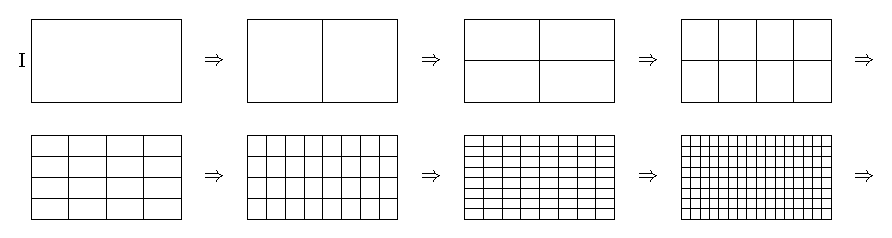
\includegraphics[width=0.9\textwidth]{MA4L2_1.eps}
		\caption{Измельчение $\MI$.}
		\label{MA4L2_1}
	\end{figure}
	Тогда $\exists \, k \colon \MI_m^{N+1} \subset \MI_k^{N}, \, \forall m \neq l, \, \MI_m^N \cap \MI_l^N = \VN$ и $\diam(\MI_m^N) < \tfrac{1}{N}$. Предъявим последовательность функций:
	$$
		h_N(x) = \ddsum{m}{} \inf\limits_{\MI_m^N}f(x){\cdot}\chi_{\MI_m^N}(x), \quad 	g_N(x) = \ddsum{m}{} \sup\limits_{\MI_m^N}f(x){\cdot}\chi_{\MI_m^N}(x)
	$$
	Отличие от сумм Дарбу здесь в том, что бруски не пересекаются $\Rightarrow$ это не обычное разбиение, как в определении интеграла, а разбиение чуть более общее (это сделано, чтобы не было наложений значений). Проверим свойства из теоремы:
	\begin{enumerate}[label=\arabic*)]
		\item $h_N(x) \leq h_{N+1}(x)$, поскольку бруски не пересекаются, то тут всегда только одно слагаемое может быть не $0$, разбили брусок на мелкие и только один мелкий будет содержать $x$, тем самым: 
		$$
			h_N(x) = \inf\limits_{\MI_m^N}f(x), \; h_{N+1}(x) = \inf\limits_{\MI_k^{N+1}}f(x)
		$$
		\begin{figure}[H]
			\centering
			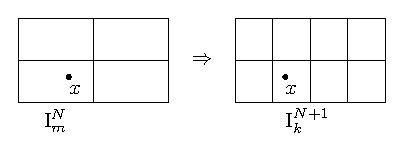
\includegraphics[width=0.4\textwidth]{MA4L2_2.eps}
			\caption{Измельчение относительно конкретной точки $x$.}
			\label{MA4L2_2}
		\end{figure}
		При измельчении точная нижняя грань не уменьшается, тогда:
		$$
			x \in \MI_{m}^N \wedge x \in \MI_k^{N+1} \Rightarrow \MI_k^{N+1} \subset \MI_{m}^N \Rightarrow h_N(x) = \inf\limits_{\MI_m^N}f(x) \leq \inf\limits_{\MI_k^{N+1}}f(x) = h_{N+1}(x)
		$$
		Для $g_N(x)$ получется аналолгично: $g_N(x) \geq g_{N+1}(x)$;
		\item $h_N(x) \leq f(x) \leq g_N(x)$ - очевидно, поскольку $h_N(x)$ - точная нижняя грань $f(x)$ на соответствующем бруске, $g_N(x)$ - точная верхняя грань $f(x)$ на соответствующем бруске;
		
		\item Воспользуемся результатами предыдущих пунктов, тогда:
		$$
			0 \leq \ddint{\MI}{}g_N(x)dx - \ddint{\MI}{}h_N(x)dx = \ddsum{m}{}\sup\limits_{\MI_m^N}f(x){\cdot}\left|\MI_m^N\right| -  \ddsum{m}{}\inf\limits_{\MI_m^N}f(x){\cdot}\left|\MI_m^N\right| 
		$$
		Для простоты дальнейших рассуждений замкнём бруски (для определения интеграла Римана). Когда мы замыкаем, мы увеличиваем множество и $\sup$ может только возрасти, а $\inf$ может только уменьшиться, тогда:
		$$	
			\ddsum{m}{}\left(\sup\limits_{\MI_m^N}f(x) - \inf\limits_{\MI_m^N}f(x)\right){\cdot}\left|\MI_m^N\right| \leq \ddsum{m}{}\left(\sup\limits_{\ovl{\MI}_m^N}f(x) - \inf\limits_{\ovl{\MI}_m^N}f(x)\right){\cdot}\left|\ovl{\MI}_m^N\right|
		$$
		Заметим, что $\ovl{\MTB}^N = \left\{\ovl{\MI}_m^N\right\}$ - разбиение $\MI$ такое, что: $\lambda\left(\ovl{\MTB}^N\right) < \tfrac{1}{N}$, поскольку добавление границы длины брусков поменять не может. Поскольку $f$ - интегрируема, тогда:
		$$
			\forall \xi^N, \, \left|\sigma\left(f,\ovl{\MTB}^N, \xi^N\right) - \ddint{\MI}{}f(x)dx \right| \xrightarrow[N \to \infty]{} 0
		$$
		Пусть $\VE > 0$, выберем $\xi^N$ и $\wte{\xi}^N$ так, чтобы: $f(\xi_m^N) < \inf\limits_{\ovl{\MI}_m^N}f(x) + \VE$ и $f(\wte{\xi}_m^N) > \sup\limits_{\ovl{\MI}_m^N}f(x) - \VE$, тогда:
		$$
			0 \leq \ddint{\MI}{}g_N(x)dx - \ddint{\MI}{}h_N(x)dx \leq \sigma\left(f,\ovl{\MTB}^N, \wte{\xi}^N\right) - \sigma\left(f,\ovl{\MTB}^N, \xi^N\right) + 2\VE{\cdot}|\MI| \xrightarrow[N \to \infty]{} 0 + 2\VE{\cdot}|\MI| = 2\VE{\cdot}|\MI|
		$$
		Поскольку $\VE$ можно сделать сколь угодно маленьким, то будет верно:
		$$
			\ddint{\MI}{}g_N(x)dx - \ddint{\MI}{}h_N(x)dx \xrightarrow[N \to \infty]{} 0
		$$
	\end{enumerate}
\end{proof}
\begin{rem}
	Для любой ограниченной функции $f$ на $\MI$ всегда $\exists\, h_n, g_n \colon h_n \leq h_{n+1}, \, g_n \geq g_{n+1}, \, h_n \leq f \leq g_n$.
\end{rem}
\begin{rem}
	Для любой интегрируемой функции $f$ на $\MI$ к предыдущему замечанию добавляется, что:
	$$
		\ddint{\MI}{}h_n(x)dx - \ddint{\MI}{}g_n(x)dx \to 0
	$$
\end{rem}
\begin{rem}
	Можно рассматривать только построенные последовательности: 
	$$
		h_N(x) = \ddsum{m}{} \inf\limits_{\MI_m^N}f(x){\cdot}\chi_{\MI_m^N}(x), \quad g_N(x) = \ddsum{m}{} \sup\limits_{\MI_m^N}f(x){\cdot}\chi_{\MI_m^N}(x)
	$$ 
	Тогда: 
	$$
		f \text{ - интегрируема } \Leftrightarrow \ddsum{m}{}\left(\sup\limits_{\MI_m^N}f(x)  - \inf\limits_{\MI_m^N}f(x)\right){\cdot}|\MI_m^N| \xrightarrow[N \to \infty]{} 0
	$$
	Почти критерий Дарбу, отличие в том, что мы не рассматриваем суммы Дарбу, а рассматриваем последовательности вложенных разбиений $\Rightarrow$ нельзя написать для любого разбиения, масштаб которого стремится к нулю верно, что разность выше тоже стремится к нулю, где можно было бы заменить:
	$$
		\omega\left(f,\MI_m^N\right) = \sup\limits_{\MI_m^N}f(x)  - \inf\limits_{\MI_m^N}f(x)
	$$
\end{rem}
\begin{rem}
	В доказательстве достаточности нам не важно, что функции ступенчатые, но в необходимости мы строим ступенчатые. Также заметим, что из ступенчатости следует их интегрируемость.
\end{rem}

\subsection*{Теорема Фубини}
\begin{defn}
	\uwave{Повторным интегралом Римана} называются интегралы вида:
	$$
		\int\limits_{\MI_x}\Bigg(\int\limits_{\MI_y}f(x,y)dy\Bigg)dx, \quad \int\limits_{\MI_y}\Bigg(\int\limits_{\MI_x}f(x,y)dx\Bigg)dy
	$$
\end{defn}

\begin{theorem}(\textbf{Фубини})
	Пусть $\MI = \MI_x \times \MI_y$, $\MI_x \subset \MR^n, \, \MI_y \subset \MR^m$ - замкнутые бруски (в том числе $\MI$ тоже замкнутый брусок). Пусть $f$ интегрируема по Риману на $\MI$ и $\forall x \in \MI_x$ функция $y \mapsto f(x,y)$ интегрируема на бруске $\MI_y$, тогда функция: $x \mapsto \int_{\MI_y}f(x,y)dy$ интегрируема на $\MI_x$ и верно равенство:
	$$
		\iint\limits_{\MI} f(x,y)dxdy = \int\limits_{\MI_x}\Bigg(\int\limits_{\MI_y}f(x,y)dy\Bigg)dx
	$$
	Если $\forall y \in \MI_y$ функция $x \mapsto f(x,y)$ интегрируема на бруске $\MI_x$, тогда функция: $y \mapsto \int_{\MI_x}f(x,y)dx$ интегрируема на $\MI_y$ и верно равенство:
	$$
		\iint\limits_{\MI} f(x,y)dxdy = \int\limits_{\MI_y}\Bigg(\int\limits_{\MI_x}f(x,y)dx\Bigg)dy
	$$
\end{theorem}
\begin{rem}
	По теореме Фубини, если у нас есть брусок $\MI =  \MI_x \times \MI_y$ и мы хотим проинтегрировать функцию $f(x,y)$ по нему. Для этого, мы фиксируем каждый раз точку $x$ и интегрируем по сечению, то есть интегрируем по $y$. И таким образом мы можем зафиксировать все $x$ вдоль $\MI_x$.
	\begin{figure}[H]
		\centering
		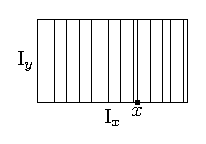
\includegraphics[width=0.25\textwidth]{MA4L2_3.eps}
		\caption{Интегрирование по $\MI_x$.}
		\label{MA4L2_3}
	\end{figure}
	Получаем функцию, которая выдаёт значения интегралов на сечении, затем мы эту функцию проинтегрируем по $x$, то есть ``сложим'' все эти сечения.
\end{rem}
\begin{rem}
	В одномерном случае интеграл это попытка посчитать площадь под графиком, здесь же многомерный интеграл это попытка посчитать объем под графиком.
	\begin{figure}[H]
		\centering
		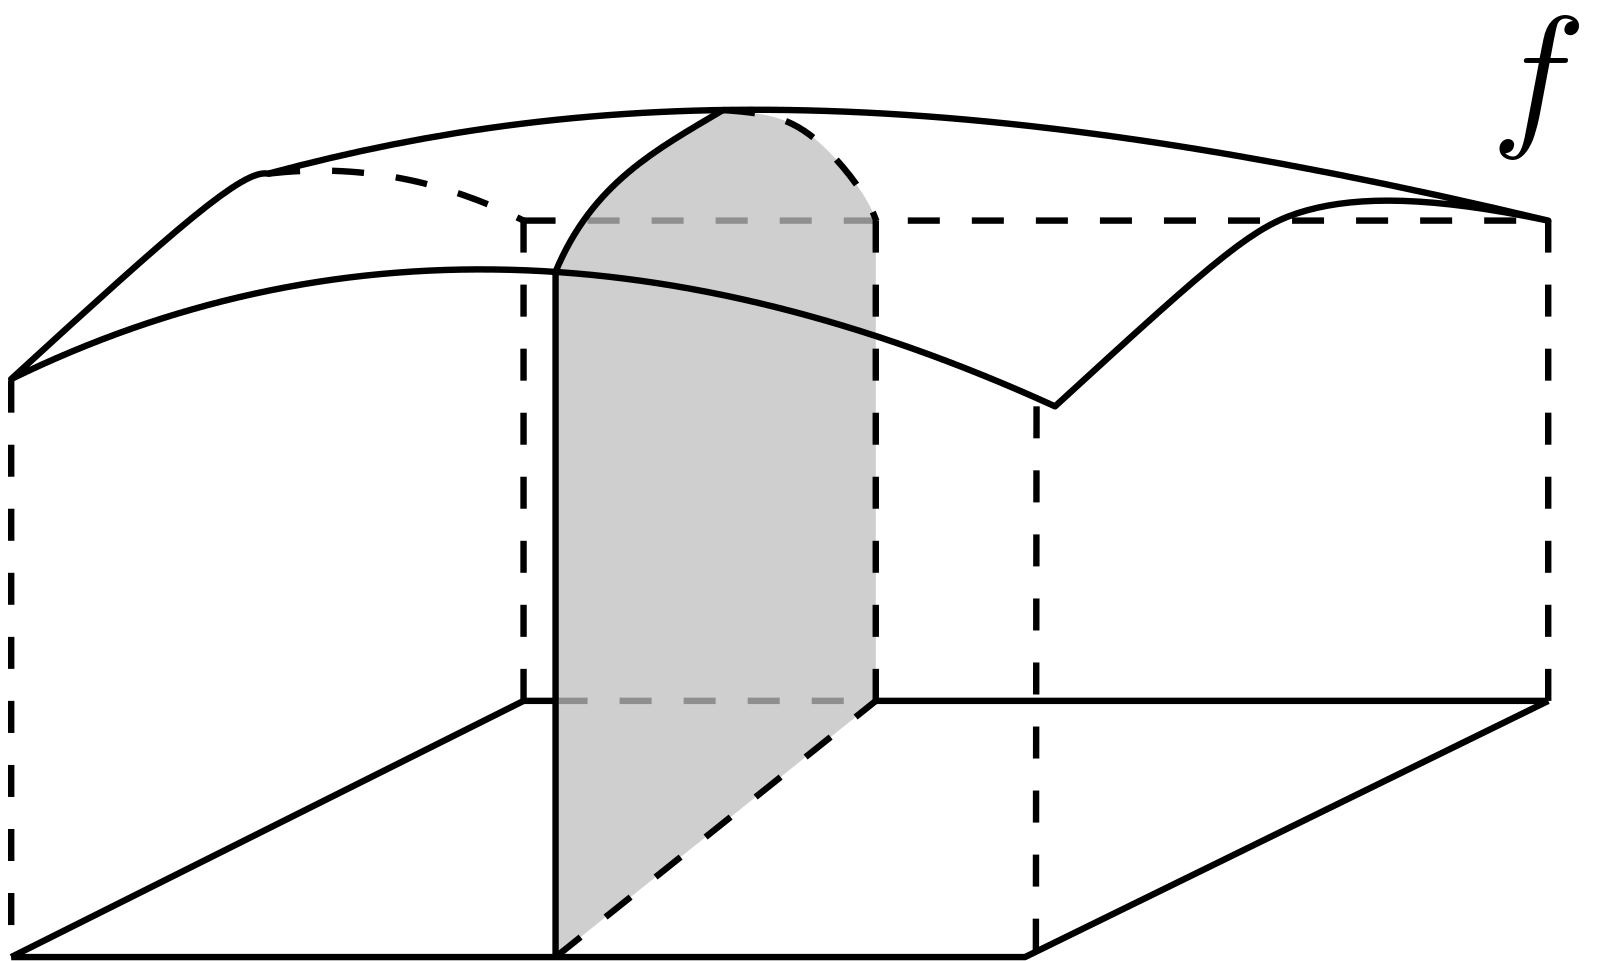
\includegraphics[width=0.3\textwidth]{MA4L2_4.png}
		\caption{Площадь сечения под графиком.}
		\label{MA4L2_4}
	\end{figure}
	Она предлагает брать сечения под графиком, считать их площадь и складывать $\Rightarrow$ смотрим на сечения.
\end{rem}
\begin{problem}
	Что будет в пересечении двух трубок одинакового диаметра под прямым углом?
	\begin{figure}[H]
		\centering
		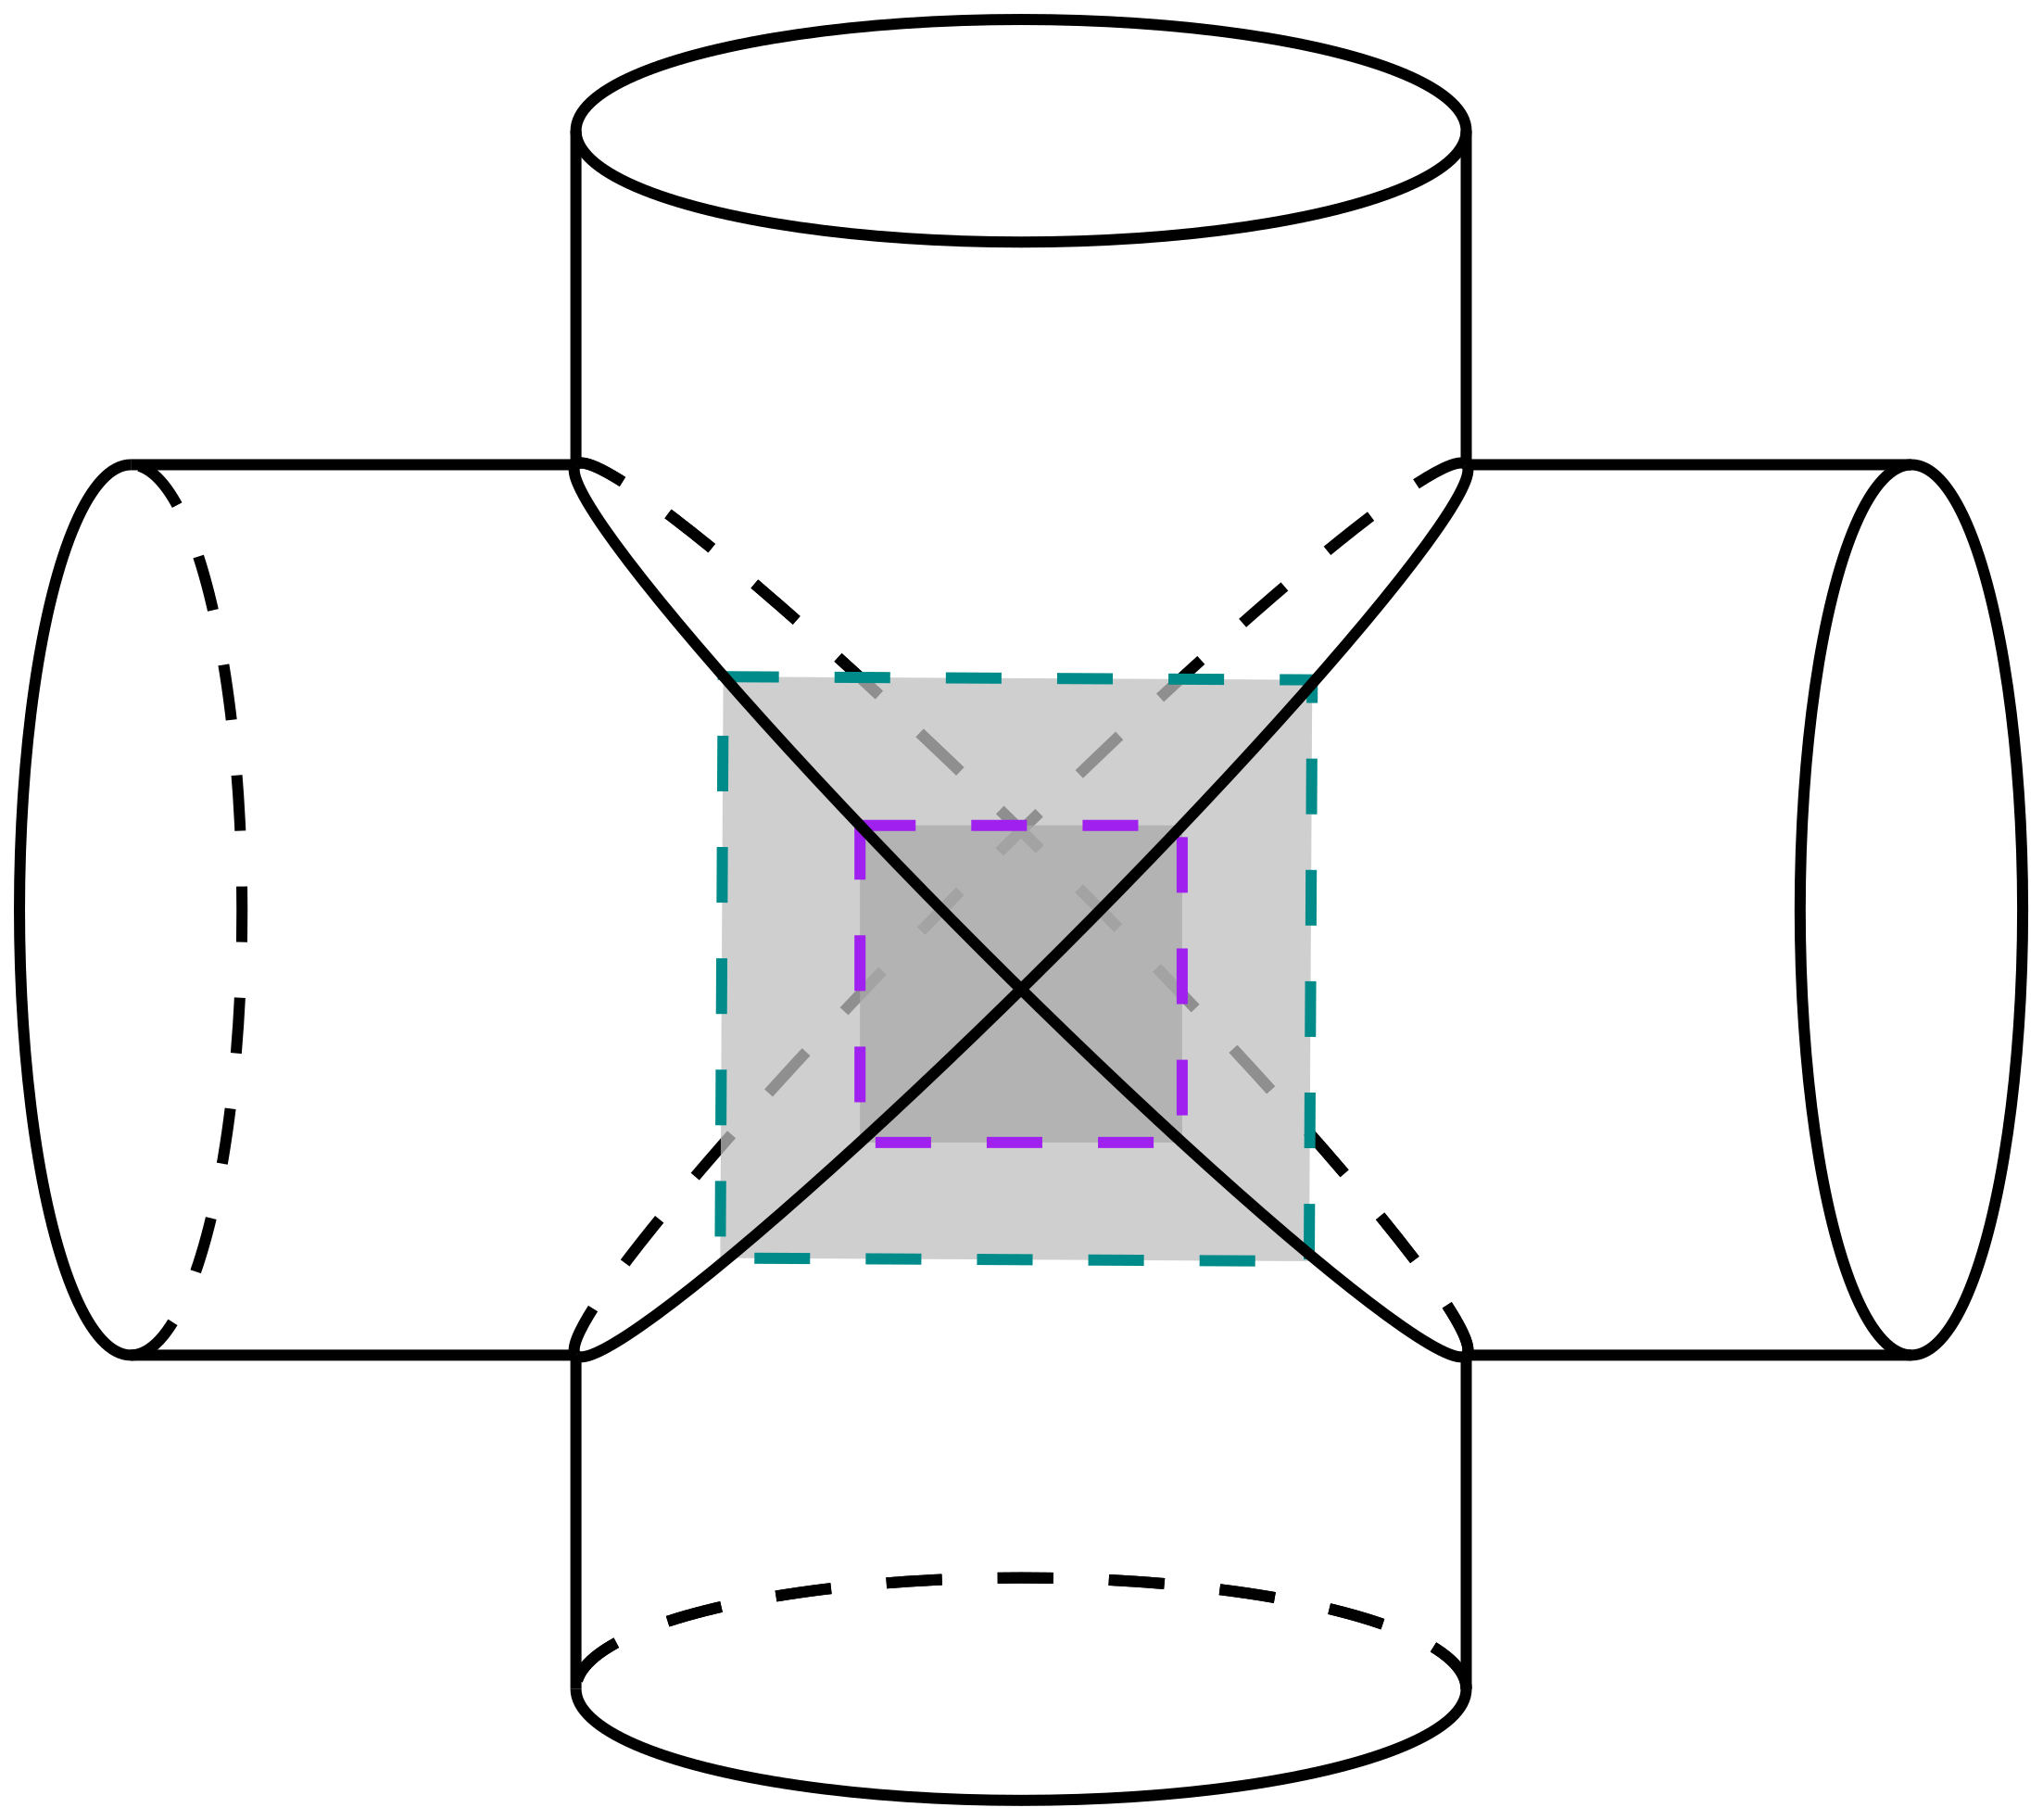
\includegraphics[width=0.3\textwidth]{MA4L2_5.png}
		\caption{Пересечение двух трубок под прямым углом.}
		\label{MA4L2_5}
	\end{figure}
\end{problem}
\begin{proof}
	Можно считать, что трубки получились из уравнений: $x^2 + y^2 \leq 1$ и $x^2 + z^2 \leq 1$, тогда:
	$$
		|y| \leq \sqrt{1 - x^2} ,\, |z| \leq \sqrt{1 - x^2}
	$$
	Таким образом, если мы возьмём сечения при фиксированном $x$, будут получаться квадраты.
\end{proof}
Аналогичный вопрос может быть про четырехмерный куб: $[0,1]^4$, как его себе представить? Один из способов это посмотреть сечения. Многомерные объекты мы так и понимаем - с помощью сечений.

В формулировке есть очень важное условие от которого отказаться нельзя: $\forall x \in \MI_x$ функция $y \mapsto f(x,y)$ интегрируема на бруске $\MI_y$. 

\textbf{Пример}: рассмотрим следующую функцию:
$$
	f(x,y) = 
	\begin{cases}
		0, & x \neq \tfrac{1}{2}\\
		D(y), & x = \tfrac{1}{2}
	\end{cases}
$$
где $D(x)$ - функция Дирихле. По определению это интегрируемая функция, поскольку какое бы разбиение ни взяли, в Римановой сумме отлично от нуля лишь слагаемое, где задето сечение $x = \tfrac{1}{2}$, но сумма объемов этих слагаемых не превосходит $2 \lambda(\MTB)$ и следовательно: $\sigma \to 0$. Но в $x = \tfrac{1}{2}$ функция Дирихле и никакого интеграла по $y$ не существует и такое может происходить не только на одном сечении. Поэтому исключив требование выше, интеграла по $\MI_y$ не будет.

После доказательства можно будет обсудить, как хитро доопределять $f(x,y)$ в тех $x$ для которых функция не интегрируема, но отметим, что интеграл Римана плохо реагирует на переопределения. Чтобы не перегружать теорему, мы пока обойдемся без этого. Аналогичное требоване есть, если расписываем всё в другом порядке.

Также отметим, что в обратную сторону теорема не верна: может так случиться, что у функции всё отлично на каждом сечении (как по $x$, так и по $y$), но при этом интеграла по квадрату нет (например, построив аналог функции Дирихле на квадрате: на плотном множестве $1$, а вне него $0$ так, чтобы на каждом сечении 
эта функция будет либо $0$, либо только в одной точке будет $\neq 0$).

\subsection*{Доказательство теоремы Фубини}
\begin{proof}
	Пусть $\MJ \subset \MI = \MI_x \times \MI_y$ - произвольный брусок. Верно: $\MJ = \MJ_x \times \MJ_y$, поскольку брусок это произведение отрезков, а лююбой подбрусок это выбор в каждом отрезке промежутка и их перемножение. Рассмотрим индикаторы: $\chi_{\MJ}(x,y) = \chi_{\MJ_x}(x){\cdot}\chi_{\MJ_y}(y)$ - как мы установлии в прошлый раз. Рассмотрим интегралы:
	$$
		 \ddint{\MI}{}\chi_{\MJ}(x,y)dxdy = |\MJ| 
	$$
	$$
		 \ddint{\MI_x}{}\bigg(\ddint{\MI_y}{}\chi_{\MJ}(x,y)dy\Bigg)dx = \ddint{\MI_x}{}\bigg(\ddint{\MI_y}{}\chi_{\MJ_x}(x){\cdot}\chi_{\MJ_y}(y)dy\Bigg)dx =	\ddint{\MI_x}{}\chi_{\MJ_x}(x){\cdot}\Bigg(\ddint{\MI_y}{}\chi_{\MJ_y}(y)dy\Bigg)dx = 
	$$
	$$
		= \ddint{\MI_x}{}\chi_{\MJ_x}(x){\cdot}|\MJ_y|dx = |\MJ_y|{\cdot}\ddint{\MI_x}{}\chi_{\MJ_x}(x)dx = |\MJ_x|{\cdot}|\MJ_y| = |\MJ|
	$$
	Тоже самое верно и в другом порядке. Следовательно, для ступенчатой функции теорема верна. Воспользуемся критерием интегрируемости, тогда: $\exists$ последовательность $h_n(x,y), \, g_n(x,y)$ ступенчатых функций, для которых выполняются свойства:
	\begin{enumerate}[label=\arabic*)]
		\item $h_n(x,y) \leq f(x,y) \leq g_n(x,y),\, \forall n$;
		\item $h_n(x,y) \leq h_{n+1}(x,y); \,  g_{n+1}(x,y) \leq g_n(x,y),\, \forall n$;
		\item $\int_{\MI}{}g_n(x,y)dxdy - \int_{\MI}{}h_n(x,y)dxdy \xrightarrow[n \to \infty]{} 0$;
	\end{enumerate}
	Отметим, что функция $H_n(x) = \int_{\MI_y}h_n(x,y)dy$ будет снова ступенчатой функцией, поскольку она равна индикатору бруска по $x$, умноженному на число. Аналогично для $G_n(x) = \int_{\MI_y}g_n(x,y)dy$. Подробнее:
	$$
		h_n(x,y) = \ddsum{k}{}c_k{\cdot}\chi_{\MJ_k}(x,y) \Rightarrow \ddint{\MI_y}{}h_n(x,y)dy = \ddsum{k}{}c_k{\cdot}|\MJ_{k,y}|{\cdot}\chi_{\MJ_{k,x}}(x) = \ddsum{k}{}\wte{c_k}{\cdot}\chi_{\MJ_{k,x}}(x)
	$$
	Нам необходимо доказать интегрируемость функции $x \mapsto \int_{\MI_y}f(x,y)dy$ на $\MI_x$ и равенство двойного интеграла повторному. Для этого потребуется воспользоваться критерием интегрируемости. 
	
	По монотонности интеграла понятно, что $H_n$ не убывает, а $G_n$ не возрастает и по этой же причине верно:
	$$
		h_n(x,y) \leq f(x,y) \leq g_n(x,y) \Rightarrow H_n(x) \leq \ddint{\MI_y}{}f(x,y)dy \leq G_n(x)
	$$
	Рассмотрим интегралы для $H_n(x), \, G_n(x)$ и применим уже доказанное выше для ступенчатых функций:
	$$
		\ddint{\MI_x}{}H_n(x)dx = \ddint{\MI_x}{}\Bigg(\ddint{\MI_y}{}h_n(x,y)dy   \Bigg)dx = \iint\limits_{\MI}{}h_n(x,y)dxdy \xrightarrow[n \to \infty]{} \iint\limits_{\MI}{}f(x,y)dxdy
	$$
	$$
		\ddint{\MI_x}{}G_n(x)dx = \ddint{\MI_x}{}\Bigg(\ddint{\MI_y}{}g_n(x,y)dy   \Bigg)dx = \iint\limits_{\MI}{}g_n(x,y)dxdy  \xrightarrow[n \to \infty]{} \iint\limits_{\MI}{}f(x,y)dxdy
	$$
	Следовательно, разности этих интегралов, а значит и разность интегралов от $H_n$ и $G_n$ стемятся к нулю:
	$$
		\ddint{\MI_x}{}H_n(x)dx - \ddint{\MI_x}{}G_n(x) dx \xrightarrow[n\to \infty]{} 0 \Rightarrow x \mapsto \ddint{\MI_y}{}f(x,y)dy \text{ - интегрируема}
	$$
	Кроме того: 
	$$
		\ddint{\MI_x}{}\Bigg(\ddint{\MI_y}{}f(x,y)dy \Bigg)dx = \lim\limits_{n \to  \infty}\ddint{\MI_x}{}H_n(x)dx = \iint\limits_{\MI}{}f(x,y)dxdy
	$$
\end{proof}
\begin{exrc}
	Мы использовали, что $\forall x$ существует интеграл $\int_{\MI_y}f(x,y)dy$. Как доопределять функцию в тех точках $x$ в которых этого интеграла не существует, чтобы заключение теоремы было верным? То есть:
	$$
		F(x) = 
		\begin{cases}
			\int_{\MI_y}f(x,y)dy, & \text{интеграл существует}\\
			?, & \text{интеграл не существует}
		\end{cases}
	$$
	Но так, чтобы:
	$$
		\iint\limits_{\MI}f(x,y)dxdy = \ddint{\MI_x}{}F(x)dx
	$$
	Окажется, что доопределять можно не как угодно.
\end{exrc}
\begin{exrc}
	Сколь велико множество $x$, где надо доопределять эту функцию $F(x)$?
\end{exrc}


\end{document}